%%%%%%%%%%%%%%%%%%%%%%%%%%%%%%%%%%%%%%%%%%%%%%%%%%%%%%%%%%%%%%%%%%%%%%%%%%%%
\documentclass[a4paper,10.5pt]{jsarticle}           % pLaTeX の場合
\usepackage{suri2019}
\usepackage{authblk}

\usepackage[dvipdfmx]{graphicx} 
\usepackage{amsmath,amssymb}
\usepackage{amsthm}
\usepackage{amsfonts}
%\usepackage{algorithmic}
\usepackage{algorithm}
\usepackage{algpseudocode}
\usepackage{bm}
\usepackage{color}
\usepackage{latexsym}

\newcommand{\argmax}{\mathop{\rm arg~max}\limits}
\newcommand{\argmin}{\mathop{\rm arg~min}\limits}
\usepackage{comment}

\bibliographystyle{junsrt}
%%%%%%%%%%%%%%%%%%%%%%%%%%%%%%%%%%%%%%%%%%%%%%%%%%%%%%%%%%%%%%%%%%%%%%%%%%%
\author{白川稜\Email{sira@ist.hokudai.ac.jp}
\hspace{5mm}中村篤祥 \hspace{5mm}工藤峰一\\
(北海道大学 大学院 情報科学研究科)\contactto{札幌市北区北14条西9丁目北海道大学大学院情報科学研究科}}

\title{モンテカルロ木特徴探索に基づく非線形グラフ分類回帰}

\begin{document}
\maketitle

\section{はじめに}
グラフ構造は、事物間の関係を表現することに適しているため、
様々な分野のデータ表現として用いられている。
特にケモインフォマティクスの分野では、
化学構造式やRNA二次構造などのデータの表現としてグラフを用いた研究が盛んに行われている。

本研究では、そのうちの1つとしてグラフ分類回帰問題を扱う。
グラフ分類回帰問題とは、ラベル付きグラフ集合をトレーニングデータとして与えられた際に
未知のグラフのラベルを予測する予測器を学習する問題であり、
主に創薬や材料科学分野におけるスクリーニングとしての応用がある。

本問題に利用する特徴量には一般的に部分グラフの有無(部分グラフ指示子)が挙げられるが、
部分グラフの総数はグラフサイズに対して指数関数的に増加するため特徴構築が困難である。
本研究では、回帰木を利用したアンサンブル学習モデルとモンテカルロ木特徴探索を組み合わせることで、
表現力の高い学習モデルを低コストで構築する手法を提案する。
最後に、グラフ分類回帰問題におけるベンチマークのデータを利用し、
既存手法との精度及びコスト比較の実験を考える。

\section{問題設定}
まずはじめにグラフ分類回帰問題の問題設定から記述する。
グラフ分類回帰問題は、あるグラフクラス$\mathcal{G}$上の関数
$f: \mathcal{G} \rightarrow \mathbb{N}\ or\ \mathbb{R}$
をトレーニングデータ$\mathcal{D}$から学習する問題である。
出力が離散値の場合は分類問題、実数値の場合は回帰問題となる。

\section{既存研究}
特徴量に部分グラフ指示子を利用した既存手法としてgBoost\cite{gBoost}という手法を説明する。
\subsection{モデル}
gBoostはLPBoostと呼ばれる線形計画問題によって定式化されたアンサンブル学習モデルと
木状の部分グラフ空間における探索アルゴリズムを組み合わせた手法である。
gBoostでは特徴探索とモデル構築を独立に行わずにモデル構築に必要な特徴のみを逐次的に探索する。

本手法では弱仮説に決定株(Fig.\ref{decidion_stump})を用い、弱仮説の重み付き線形和を最終的な予測器とする。
決定株の分割ルールに用いる特徴をgSpan木(Fig.\ref{search_tree})と呼ばれる部分グラフ空間を探索することで決定する。
本手法では、特徴探索においてgSpan木の親子ノードに関する包含関係を利用して有効な枝狩りを行い探索コストの削減を行う。
\begin{figure}[h]
\begin{tabular}{cc}
\begin{minipage}[t]{0.44\hsize}
\centering
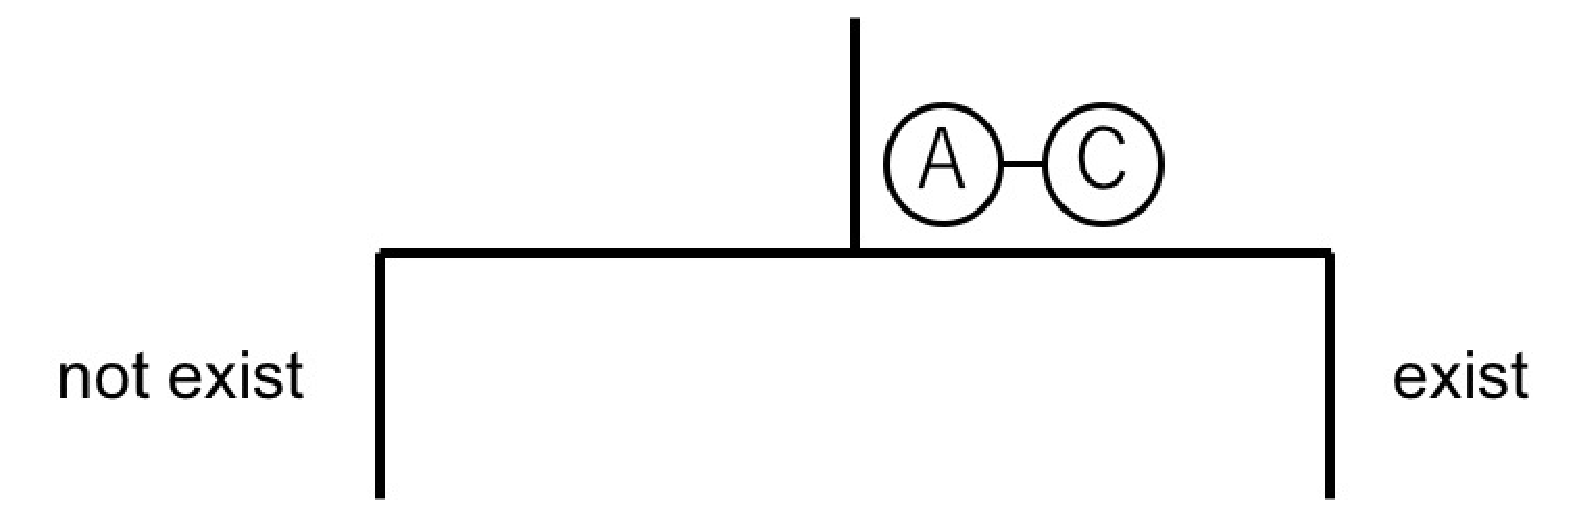
\includegraphics[width=35mm]{img/decidion_stump.eps}
\caption{決定株}
\label{decidion_stump}
\end{minipage} &
\begin{minipage}[t]{0.44\hsize}
\centering
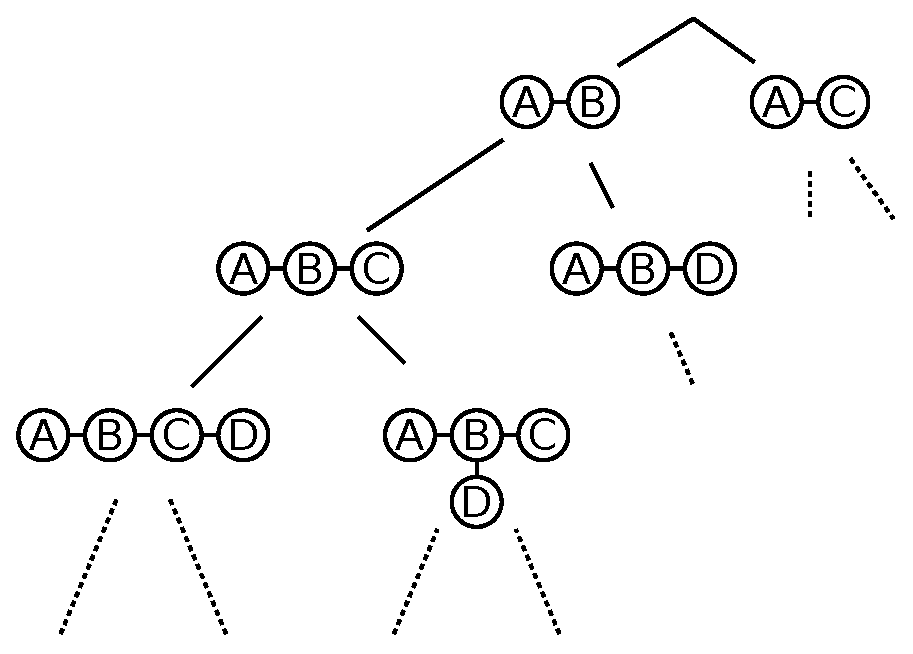
\includegraphics[width=35mm]{img/graph_search_tree.eps}
\caption{gSpan木}
\label{search_tree}
\end{minipage}
\end{tabular}
\end{figure}

\subsection{問題点}
既存手法の問題点としては以下の二点が挙げられる。
\begin{itemize}
	\item モデルの表現力
\end{itemize}
既存手法の弱仮説は決定株であり全体のモデルもその線形和で表現されるため、
既存手法は線形モデルとなる。
線形モデルは非線形モデルと比較して表現力で劣るため、学習精度の低下につながりうる。
\begin{itemize}
	\item 探索コスト
\end{itemize}
探索効率のため枝刈りを利用するが、既存手法では膨大な部分グラフ空間を厳密に探索する。
スケールの大きな問題では依然探索のコストが膨大である。

\section{提案手法}
本研究では回帰木アンサンブルモデルとモンテカルロ木探索アルゴリズムを組み合わせることで
非線形モデルを効率的に構築する手法を提案する。

\subsection{学習モデル}
提案手法では弱仮説として回帰木を用いる。
回帰木とは再帰的に集合分割を行い、集合のラベルを実数値(平均値)で予測するモデルである。
分割ルールは以下の式に従い決定される。
\begin{align}
	\argmin_{x_j \in X} [TSS(D_{1}(x_j)) + TSS(D_{0}(x_{j})] \nonumber
\end{align}
\footnotesize
\begin{align}
	X:全部分グラフ集合,\ TSS: 二乗誤差和, \nonumber
\end{align}
\begin{align}
	 D_{1}(x_j):\{x_{j}を含むグラフ集合\},\ D_{0}(x_j):\{x_{j}を含まないグラフ集合\}\nonumber
\end{align}
\normalsize

回帰木は非線形モデルであり決定株よりも表現力の高いモデルである。
また勾配ブースティングによりアンサンブルを取ることで精度及び安定性の向上を図る。

\subsection{モンテカルロ木探索}
本手法では弱学習器を回帰木に拡張したことにより集合分割の回数が既存手法よりも増加する。

そこで本手法ではモンテカルロ木探索により特徴探索を行うことで一度の探索におけるコストの削減を図る。
モンテカルロ木探索\cite{mcts_survey}\cite{fuse}とは
モンテカルロシミュレーションと解の評価値のの見積もりをうまく組み合わせた強化学習の一つであり、
膨大な探索空間から限られたコスト内でより良い解が得られる手段として注目されている。

本探索ではモンテカルロ木探索の一種であるUCTアルゴリズムを利用し分割特徴を決定する。
UCTアルゴリズムは大きく分けて4つの操作を反復することにより探索を行う。
最終的な分割ルールはモンテカルロ木探索によって拡大される探索空間のうち、
最も回帰誤差の小さい特徴を用いる。
\begin{itemize}
	\item Selection
\end{itemize}
SelectionではUCB(Upper Confidence Bound)の値を利用して、
根ノードから各反復時点での探索空間の末端まで子ノードの選択を繰り返す。
\begin{align}
	\argmax_{c_{j} \in \{子ノード集合\} } UCB \nonumber\\
	UCB = \bar{V} + C \sqrt{2 \frac{logN}{n_{j}}} \nonumber 
\end{align}
\footnotesize
\begin{align}
	\bar{V}:c_{j}の選択による報酬平均,\ C: 探索強度パラメータ, \nonumber
\end{align}
\begin{align}
	N:親ノードの選択回数,\ n_{j}: c_{j}の選択回数, \nonumber
\end{align}
\normalsize
また本探索の報酬に関しては、$TSS$の値による回帰誤差の符号を負にしたものを利用し、
誤差が大きいほど報酬が低く誤差が小さいほど大きな報酬を得られるよう設計する。
\begin{itemize}
	\item Expansion
\end{itemize}
ExpansionではSelectionによって選択された末端ノードについて考える。
末端ノードの選択回数がある閾値を上回る際には末端ノードから子ノードを展開し各時点での探索空間に追加する。
加えて子ノードの中から1つを選択する。
\begin{itemize}
	\item Simulation
\end{itemize}
SimulationではSelection及びExpansionによって選択された
末端ノードからモンテカルロシミュレーションによりノードを展開する。
ここで愚直にgSpan木を展開するのではなく、
トレーニングデータ中の1つのグラフを無作為に選択しそのグラフ上で拡大しうるシミュレーションのみを扱うことで
1回のシミュレーションにかかるコストの削減を図る。
またシミュレーションによる拡大を制限するため、一定確率で拡大を停止する停止条件を設ける。
\begin{itemize}
	\item Backpropagation
\end{itemize}
BackpropagationではSimulationにより決定されたノードに関して報酬値を計算し、
Selectionにより選ばれたノードの報酬平均値$\bar{V}$を更新する。

\subsection{探索空間}
ここでは探索空間の形状を考える。
既存手法ではgSpan木を探索空間として利用した。
しかし、gSpan木では固有の辞書順を定め重複無しに部分グラフパターンを列挙していることから、
木全体の形が大きく偏るという特徴を持つ。
モンテカルロ木探索においてこの木の偏りは探索の偏りにつながるため、
本提案手法ではgSpan木をDAG状の空間に拡張することで探索空間の偏りを減らし探索が有効に働くよう設計する。

\begin{comment}
探索アルゴリズムの擬似コードをAlgorithm\ref{alg_search}に示す。
\begin{algorithm}
	\footnotesize 
	\caption{\small Feature Selection}\label{alg_search}
	\begin{algorithmic}[1]
		\Procedure{UCT Search}{K}
		\State グローバル変数 : $n$, $path$, $best\_subgraph$
		\For{$i=1$ to $K$}
		\State $n \gets root$
		\State \textsc{Selection}()
		\State \textsc{Expansion}()
		\State \textsc{Update}()
		\State \textsc{Simuration}()
		\State \textsc{Backpropagation}(n)
		\EndFor
		\State \textbf{return}\ $best\_subgraph$
		\EndProcedure

		\Function{Selection}{}
		\While{$n$が現探索空間における内部ノード}
		\State $path \gets path \cup n$
		\State $n \gets best\_ucb\_child \in \{nの子ノード\}$
		\EndWhile
		\State $path \gets path \cup n$
		\EndFunction

		\Function{Expansion}{}
		\If{$n$の選択回数が閾値以上}
		\State $n$の子ノードを探索空間に追加
		\State $n \gets random\_child \in \{nの子ノード\}$
		\State $path \gets path \cup n$
		\EndIf
		\EndFunction

		\Function{Update}{}
		\ForAll{$p \in \{pathの内選択が初めてのノード\}$}
		\If{$p$による分割後不純度が最良値を更新}
		\State $best\ subgraph \gets p$
		\EndIf
		\EndFor 
		\EndFunction

		\Function{Simuration}{$n$}
		\While{$n$に子ノード有り and not\ 確率的停止条件}
		\State $n \gets random\_child \in \{nの子ノード\}$
		\EndWhile
		\EndFunction

		\Function{Backpropagation}{}
		\State $n$による分割後不純度計算(報酬)
		\ForAll{$p \in path$}
		\State $update\ UCB_{p}$
		\EndFor 
		\EndFunction
	\end{algorithmic}
\end{algorithm}
\end{comment}

\section{実験}
本実験ではグラフ分類回帰問題におけるベンチマークであるQSARデータセットを用いて、
既存手法との学習精度及び学習コストの比較を行うことで、提案手法の有用性を検証する。
また、モンテカルロ木探索におけるハイパーパラメータをそれぞれ変動させ、
各ハイパーパラメータの学習結果に与える影響を調べる実験を行いたいと考える。

\section{まとめ}
回帰木アンサンブルモデルとモンテカルロ木特徴探索を組み合わせることでより軽量な非線形学習モデルを構築した。
本探索はUCTアルゴリズムによるナイーブな手法であるため、
本問題における適切なヒューリスティクスやRAVEなどの発展的な手法を取り入れることで
一層のパフォーマンスの向上が期待される。

\small 
\bibliography{all}
%\begin{thebibliography}{99}
%\bibitem{1} 情報処理北海道シンポジウム講演申込書, 1997.
%\bibitem{2} 情報処理学会北海道支部 WWWホームページ,
%http://madeira.cc.hokudai.ac.jp/RD/takai/ipsjh.html, 1997.
%\end{thebibliography}
\end{document}
%
%
% End of file: sample.tex
